\subsubsection{Sensor de turbidez}

  A turbidez foi um dos parâmetros escolhidos para o monitoramento da qualidade da água. Resumidamente este parâmetro é definido como o grau de intensidade que um feixe de luz atravessa a água, quanto menor for essa intensidade, mais sólidos em suspensão estão presentes na amostra da água analisada, logo, menor será sua qualidade, segundo a CETESB.
  
  Para medir-se este parâmetro utilizará o sensor óptico de turbidez o turbidímetro nefelométrico, que utiliza detectores fotoelétricos para medir a intensidade da luz emitida pelo próprio sensor para indicar o grau de turbidez da amostra de água.
  
  Dentre os sensores disponíveis no mercado optou-se pelo produto da empresa Ponsel, o modelo a ser utilizado é o PONSEL DIGISENS Turbidity Sensor \footnotemark, os motivos por ter escolhido este produto é sua qualidade, robustez, certificação, custo-benefício, garantia e confiabilidade da empresa.
  \footnotetext{Disponível em: <http://www.fondriest.com/ponsel-digisens-turbidity-sensor.htm>}
  
  Por se tratar de um produto importado o preço para adquirir um sensor é de R\$ 4.822,99 com impostos e frete inclusos.
  
  \begin{figure}[!h]
    \centering
    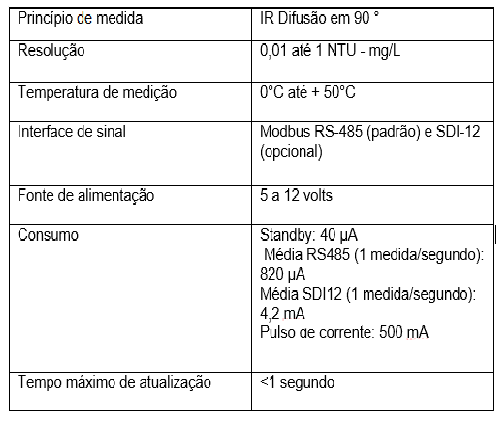
\includegraphics[scale = 0.5]{editaveis/figuras/turbidez_spec}
    \label{fishbone}
    \caption[Especificações do sensor PONSEL DIGISENS Turbidity Sensor]
      {Especificações do sensor PONSEL DIGISENS Turbidity Sensor. \footnotemark}
  \end{figure}
  \FloatBarrier
  \footnotetext{Disponível em: <http://www.fondriest.com/ponsel-digisens-turbidity-sensor.htm>}
  